\documentclass[12pt, psamsfonts]{amsart}

%-------Packages---------
\usepackage{amssymb,amsfonts}
\usepackage{semantic}
\usepackage{fullpage}
\usepackage{tikz-cd}
\usepackage{todonotes}
\usepackage{physics}
\usepackage[all,arc]{xy}
\usepackage{enumerate}
\usepackage{enumitem}
\usepackage{mathrsfs}
\usepackage{theoremref}
\usepackage{graphicx}
\usepackage[bookmarks]{hyperref}

%--------Theorem Environments--------
%theoremstyle{plain} --- default
\newtheorem{thm}{Theorem}[section]
\newtheorem{cor}[thm]{Corollary}
\newtheorem{prop}[thm]{Proposition}
\newtheorem{lem}[thm]{Lemma}
\newtheorem{conj}[thm]{Conjecture}
\newtheorem{quest}[thm]{Question}

\theoremstyle{definition}
\newtheorem{defn}[thm]{Definition}
\newtheorem{defns}[thm]{Definitions}
\newtheorem{con}[thm]{Construction}
\newtheorem{exmp}[thm]{Example}
\newtheorem{exmps}[thm]{Examples}
\newtheorem{notn}[thm]{Notation}
\newtheorem{notns}[thm]{Notations}
\newtheorem{addm}[thm]{Addendum}
\newtheorem*{exer}{Exercise}

\theoremstyle{remark}
\newtheorem{rem}[thm]{Remark}
\newtheorem{rems}[thm]{Remarks}
\newtheorem{warn}[thm]{Warning}
\newtheorem{sch}[thm]{Scholium}

\DeclareMathOperator{\Hom}{Hom}
\DeclareMathOperator{\Id}{Id}
\DeclareMathOperator{\End}{End}
\DeclareMathOperator{\ord}{ord}
\DeclareMathOperator{\Aut}{Aut}
\DeclareMathOperator{\Gal}{Gal}

\makeatletter
\let\c@equation\c@thm
\makeatother
\numberwithin{equation}{section}

\bibliographystyle{plain}

\begin{document}

\title{Qualifying Exam Prep}
\author{Hidenori Shinohara}
\maketitle

\begin{abstract}
  In order to prepare for the qualifying exam, I decided to solve problems from Hatcher and Dummit and Foote.
\end{abstract}

\tableofcontents

\section{Algebra}

\subsection{Groups}
The topics to cover: Elementary concepts (homomorphism, subgroup, coset, normal subgroup), solvable groups, commutator subgroup, Sylow theorems, structure of finitely generated Abelian groups.
Symmetric, alternating, dihedral, and general linear groups.

\subsection{Rings}
The topics to cover: Commutative rings and ideals (principal, prime, maximal).
Integral domains, Euclidean domains, principal ideal domains, polynomial rings, Eisenstein's irreducibility criterion, Chinese remainder theorem.
Structure of finitely generated modules over a principal ideal domain.

\subsubsection{Chinese remainder theorem}

\begin{exer}{(Problem 1, Section 7.6)}
  Let $R$ be a ring with identity $1 \ne 0$.
  An element $e \in R$ is called an idempotent if $e^2 = e$.
  Assume $e$ is an idempotent in $R$ and $er = re$ for all $r \in R$.
  Prove that $Re$ and $R(1 - e)$ are two-sided ideals of $R$ and that $R \cong Re \times R(1 - e)$.
  Show that $e$ and $1 - e$ are identities for the subrings $Re$ and $R(1 - e)$ respectively.
\end{exer}

\begin{proof}
  $Re$ is clearly nonempty and $re + r'e = (r + r')e \in Re$ for all $re, r'e \in Re$.
  For all $r' \in R$ and $re \in Re$, $r'(re) = (r'r)e \in Re$ and $(re)r' = r(er') = r(r'e) = (rr')e \in Re$.
  Thus $Re$ is a two-sided ideal of $R$.
  $(1 - e)^2 = 1 - e - e + e^2 = 1 - e$, and, for every $r \in R$, $r(1 - e) = r - re = r - er = (1 - e)r$.
  Thus $R(1 - e)$ is a two-sided ideal of $R$.
  Finally, $\phi: R \rightarrow R / Re \times R / R(1 - e)$ defined by $x \mapsto (x + Re, x + R(1 - e))$ is a ring homomorphism with $\ker(\phi) = Re \cap R(1 - e)$ by the Chinese Remainder Theorem.
  Let $r(1 - e) \in \ker(\phi) = Re \cap R(1 - e)$.
  Then $r(1 - e)e = r(1 - e)$ since $r(1 - e) \in Re$.
  However, this implies $r(1 - e)e = r(e - e^2) = r0 = 0$.
  Thus $\ker(\phi) = 0$, so $R \cong R / Re \times R / R(1 - e)$.
\end{proof}


\subsection{Fields Extensions}
Finite, algebraic, separable, inseparable, transcendental, splitting field of a polynomial, primitive element theorem, algebraic closure.
Finite fields.

\subsection{Galois Theory}
Finite Galois extensions and the Galois correspondence between subgroups of the Galois group and sub-extensions.
Solvable extensions and solving equations by radicals.

\begin{exer}{(Exercise 4 (Chapter 14))}
  Prove that $\mathbb{Q}(\sqrt{2})$ and $\mathbb{Q}(\sqrt{3})$ are not isomorphic.
\end{exer}

\begin{proof}
  Suppose they are and let $\phi$ be a ring isomorphism.
  $\phi(\sqrt{2}) = a + b\sqrt{3}$ for some $a, b \in \mathbb{Q}$.
  This implies $\phi(2) = (a^2 + 3b^2) + 2ab\sqrt{3}$.
  On the other hand, $\phi(2) = \phi(1) + \phi(1) = 1 + 1 = 2$.
  Thus $2ab = 0$.
  If $a = 0$, then $3b^2 = 2$, but $\sqrt{2}/3$ is not rational.
  If $b = 0$, then $a^2 = 2$, but $\sqrt{2}$ is not rational.
  This is a contradiction, so such a homomorphism does not exist.
\end{proof}

\section{Algebraic topology}

\subsection{Fundamental group}
Computation of the fundamental group, van Kampen's theorem, covering spaces.

\begin{exer}{(Exercise 8, Section 1.1)}
  Does the Borsuk-Ulam theorem hold for the torus?
\end{exer}

\begin{proof}
  No.
  Consider the natural projection map of $S^1 \times S^1$ into $\mathbb{R}^2$.
  \begin{figure}[!htb]
    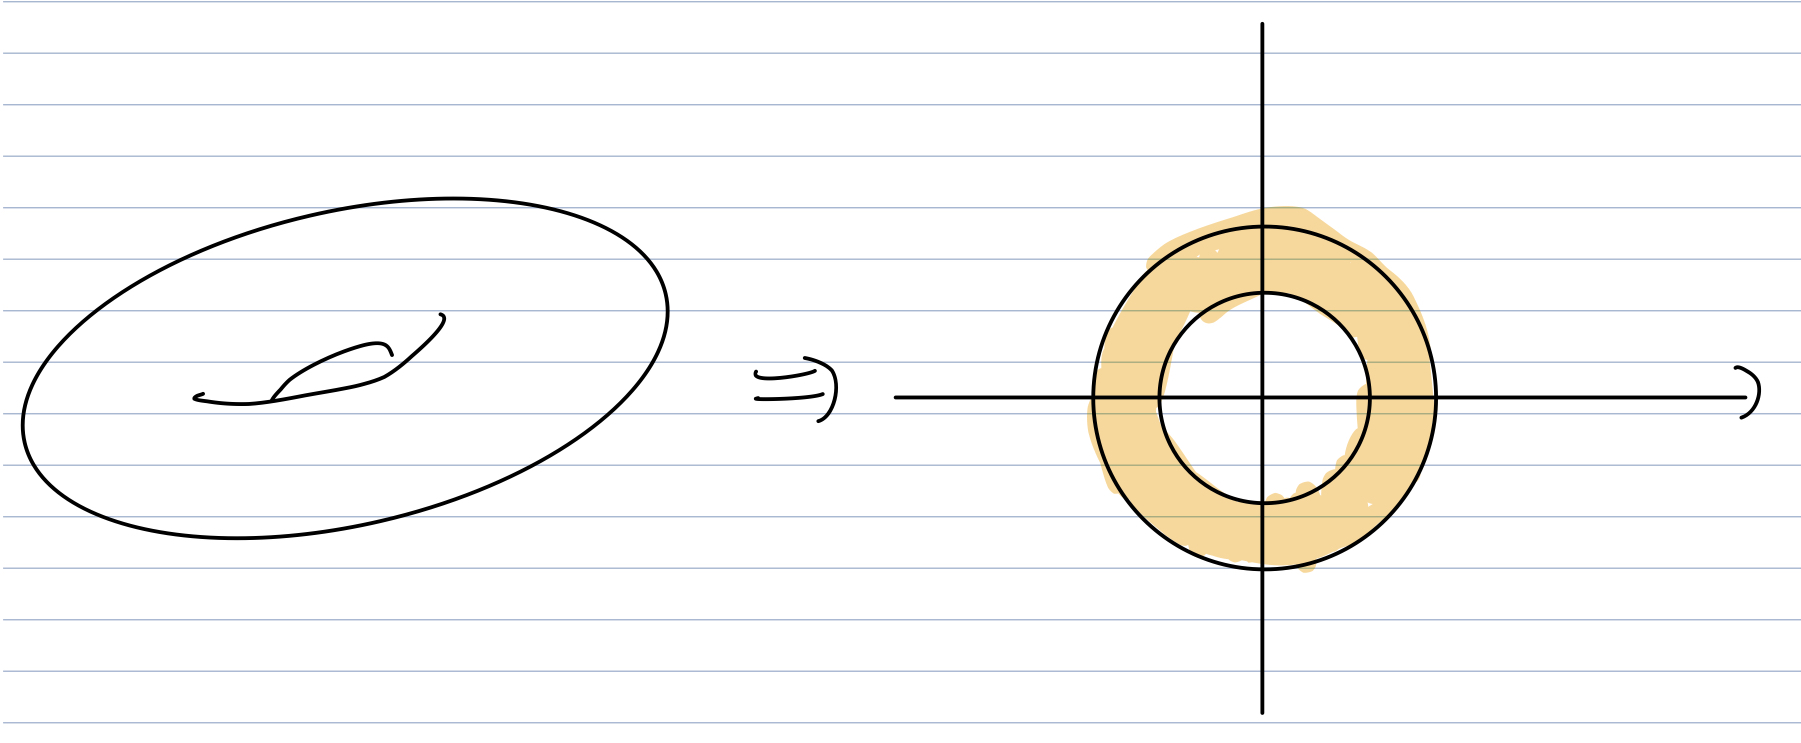
\includegraphics[width=.5\linewidth]{img/hatcher/ex-1-1-8.jpeg}
      \caption{Ex 1-1-8}
    \label{fig:ex_1_1_8}
  \end{figure}
  From Figure \ref{fig:ex_1_1_8}, it is clear that $f(x, y) = -f(-x, -y)$.
  However, $f(x, y) \ne 0$ for any $(x, y) \in S^1 \times S^1$.
  Thus $f(x, y) \ne f(-x, -y)$ for all $(x, y)$.
\end{proof}

\begin{exer}{(Exercise 2, Section 1.2)}
  Let $X \subset \mathbb{R}^m$ be the union of convex open sets $X_1, \cdots, X_n$ such that $X_i \cap X_j \cap X_k \ne \emptyset$ for all $i, j, k$.
  Show that $X$ is simply-connected.
\end{exer}

\begin{proof}
  The case that $n = 1$ is trivial.
  Suppose we have shown this for $n \in \mathbb{N}$ and let $X_1, \cdots, X_{n + 1}$ be a set of convex open sets such that the intersection of any three is nonempty.
  Let $Y = X_1 \cup \cdots \cup X_n$.
  By the inductive hypothesis, $Y$ is simply connected.
  We have
  \begin{itemize}
    \item
      $Y, X_{n + 1}$ are both path-connected open sets such that the intersection is nonempty.
    \item
      We claim that $Y \cap X_{n + 1}$ is path connected.
      Let $a, b \in Y \cap X_{n + 1}$.
      Then $a \in X_i \cap X_{n + 1}$ and $b \in X_j \cap X_{n + 1}$ for some $i, j \in \{ 1, \cdots, n \}$.
      Then $X_i \cap X_j \cap X_{n + 1}$ is nonempty, and choose a point $y$ in the intersection.
      Then $a$ and $y$ can be joined by a path because $X_i \cap X_{n + 1}$ is convex.
      Similarly, $b$ and $y$ can be joined by a path.
      Therefore, $a$ and $b$ can be joined by a path, so $Y \cap X_{n + 1}$ is path connected.
  \end{itemize}
  By the van Kampen theorem, $\pi_1(X) \cong \pi_1(Y) * \pi_1(X_{n + 1}) / N$ for some normal subgroup $N$.
  However, it does not matter what $N$ is because $\pi_1(Y)$ and $\pi_1(X_{n + 1})$ are both trivial.
  Thus $\pi_1(X) = 1$.
\end{proof}

\subsection{Homology}
Singular chains, chain complexes, homotopy invariance.
Relationship between the first homology and the fundamental group, relative homology.
The long exact sequence of relative homology.
The Mayer-Vietoris sequence.

\begin{exer}{(Exercise 1, Section 2.1)}
  What familiar space is the quotient $\Delta$-complex of a 2-simplex $[v_0, v_1, v_2]$ obtained by identifying the edges $[v_0, v_1]$ and $[v_1, v_2]$, preserving the ordering of vertices?
\end{exer}

\begin{proof}
  \begin{figure}[!htb]
    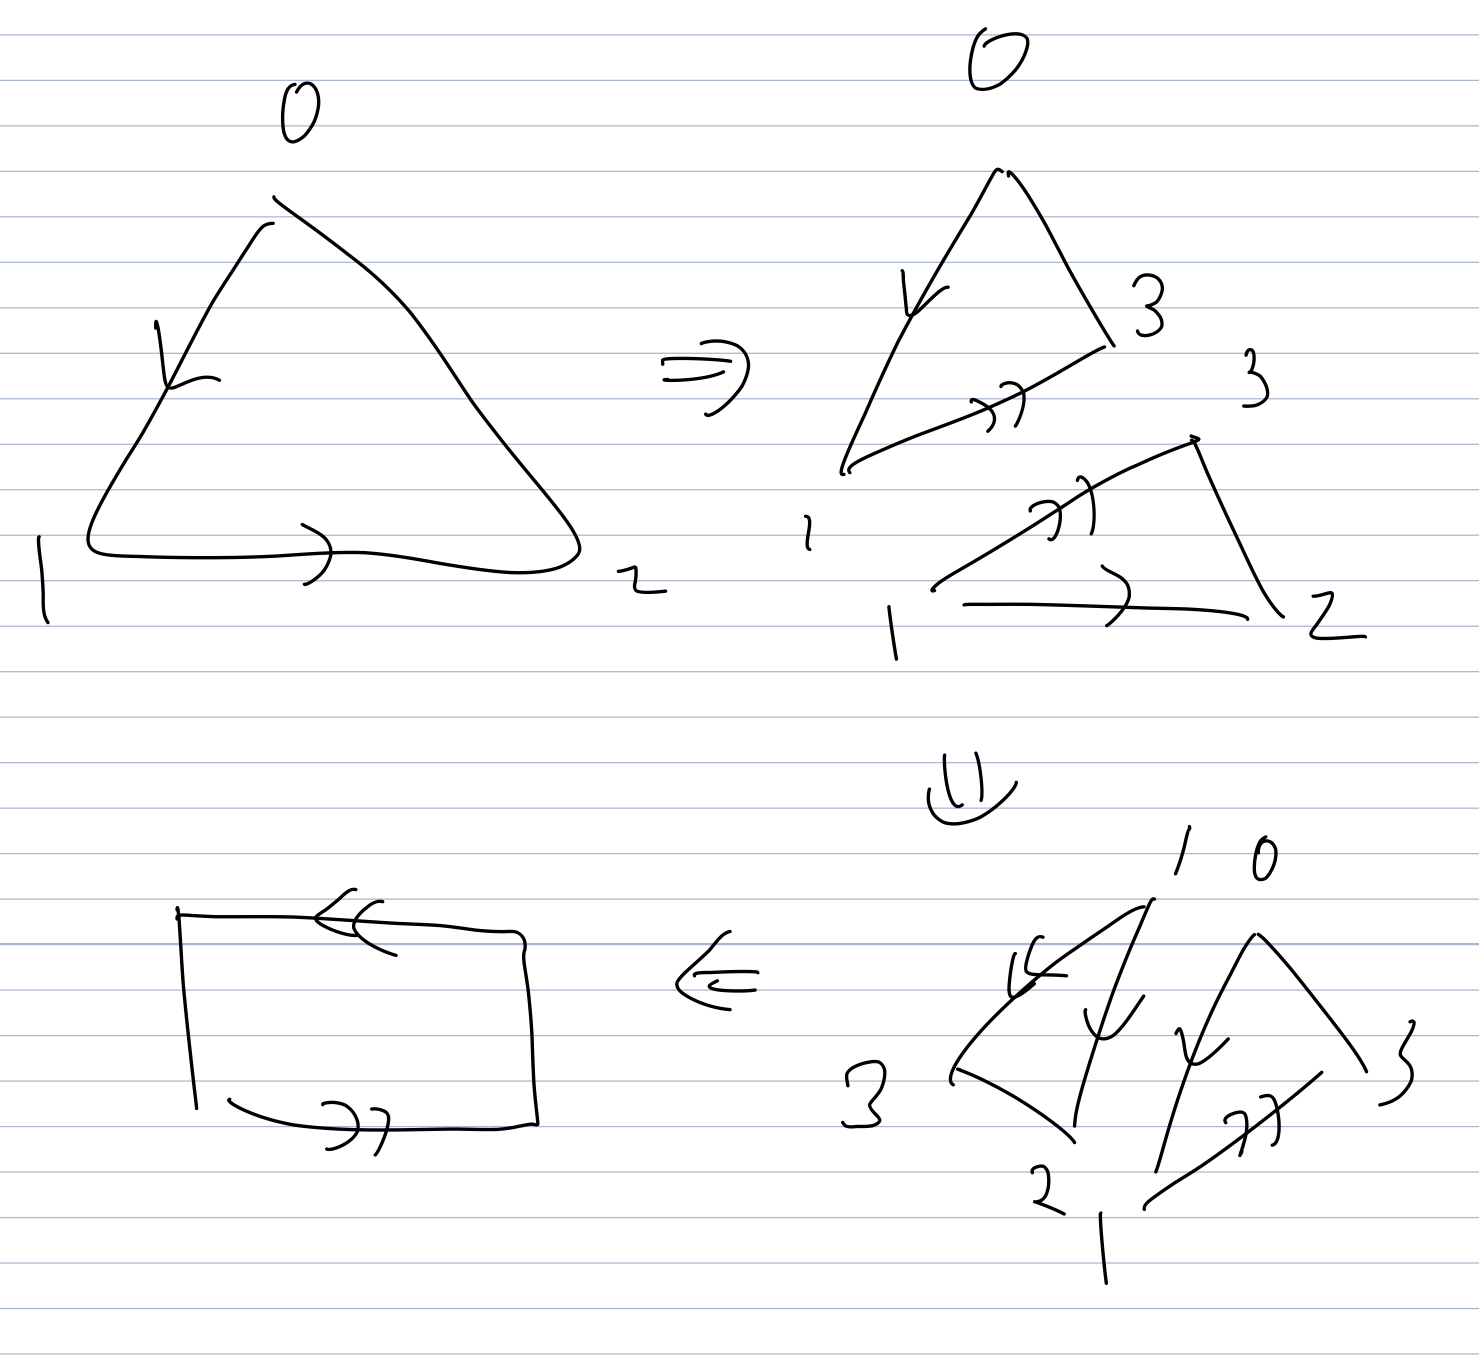
\includegraphics[width=.5\linewidth]{img/hatcher/ex-2-1-1.jpeg}
    \caption{Ex 2-1-1}
    \label{fig:ex_2_1_1}
  \end{figure}

  This can be seen easily if we cut the triangle in half and rotate one of the pieces as shown in \ref{fig:ex_2_1_1}.
  This space is a Mobius band.
\end{proof}


\end{document}


